\chapter{Markov chains}

\section{Rewriting the recurrence relation}
If we define the row vector of state probabilities at time $n$ as $\mu_{n}$ and
the stochastic matrix as $\mathcal{P}$, we can write
\begin{equation}
  \mu_{n} = \mu_{n-1} \mathcal{P}.
\end{equation}
The $(i, j)$-th entry of $\mathcal{P}$, $p_{ij}$, is the probability to go from
state $i$ to state $j$. If we work out the vector-matrix product in the previous
formula, we get, for state $i$,
\begin{equation}
  \mu_{n}(i) = \sum_{j \in S} p_{ji} \mu_{n-1}(j),
\end{equation}
where $S$ denotes the set of possible states. Then, we can split the sum and
obtain
\begin{equation}
  \mu_{n}(i) = p_{ii} \mu_{n-1}(i) + \sum_{j \neq i} p_{ji} \mu_{n-1}(j).
\end{equation}
The first term is representative of the situation in which the system was in the
same state $i$ at time $n-1$, while the second represents all the possible
transitions from another state to $i$. We can also rewrite the first term using
the fact that the rows of the stochastic matrix are normalized:
\begin{equation}
  \sum_{j \in S} p_{ij} = 1 \implies p_{ii} = 1 - \sum_{j \neq i} p_{ij}.
\end{equation}
In this way we obtain the formula we needed to prove,
\begin{equation}
  \mu_{n}(i) = \biggl(1 - \sum_{j \neq i} p_{ij}\biggr)
  \, \mu_{n-1}(i) + \sum_{j \neq i} p_{ji} \mu_{n-1}(j).
\end{equation}

\section{Drawing digraphs}

Below is the set of directed graphs corresponding to the given stochastic
matrices.

\bigskip
\noindent
\begin{minipage}[c]{0.5\textwidth}
  \centering
  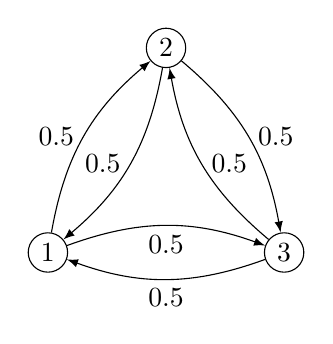
\begin{tikzpicture}[
    vertex/.style={circle, draw, minimum size=0.5cm, inner sep=0pt},
    baseline=(current bounding box.center),
    ]
    \node[vertex] (1) at (0, 0) {$1$};
    \node[vertex] (2) at (1.5, {1.5 * sqrt(3)}) {$2$};
    \node[vertex] (3) at (3, 0) {$3$}; 

    \draw[-latex] (1) to[bend left=20] node[left] {$0.5$} (2);
    \draw[-latex] (1) to[bend left=20] node[below] {$0.5$} (3);
    \draw[-latex] (2) to[bend left=20] node[left] {$0.5$} (1);
    \draw[-latex] (2) to[bend left=20] node[right] {$0.5$} (3);
    \draw[-latex] (3) to[bend left=20] node[below] {$0.5$} (1);
    \draw[-latex] (3) to[bend left=20] node[right] {$0.5$} (2);
  \end{tikzpicture}
\end{minipage}%
\begin{minipage}[c]{0.5\textwidth}
  \begin{equation}
    \mathcal{P} =
    \begin{pmatrix}
      0  & 0.5 & 0.5 \\
      0.5 &  0  & 0.5 \\
      0.5 & 0.5 &  0
    \end{pmatrix}
  \end{equation}
\end{minipage}

\noindent
\begin{minipage}[c]{0.5\textwidth}
  \centering
  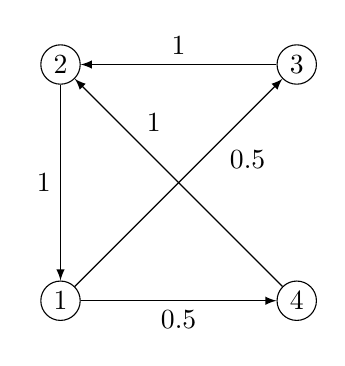
\begin{tikzpicture}[
    vertex/.style={circle, draw, minimum size=0.5cm, inner sep=0pt},
    baseline=(current bounding box.center),
  ]
    \node[vertex] (1) at (0, 0) {$1$};
    \node[vertex] (2) at (0, 3) {$2$};
    \node[vertex] (3) at (3, 3) {$3$};
    \node[vertex] (4) at (3, 0) {$4$};

    \draw[-latex] (1) to node[pos=0.7, below right] {$0.5$} (3);
    \draw[-latex] (1) to node[below] {$0.5$} (4);
    \draw[-latex] (2) to node[left] {$1$} (1);
    \draw[-latex] (3) to node[above] {$1$} (2);
    \draw[-latex] (4) to node[pos=0.7, above right] {$1$} (2);
  \end{tikzpicture}
\end{minipage}%
\begin{minipage}[c]{0.5\textwidth}
  \begin{equation}
    \mathcal{P} = 
    \begin{pmatrix}
      0 & 0 & 0.5 & 0.5 \\
      1 & 0 &  0  &  0  \\
      0 & 1 &  0  &  0  \\
      0 & 1 &  0  &  0
    \end{pmatrix}
  \end{equation}
\end{minipage}

\bigskip
\noindent
\begin{minipage}[c]{0.55\textwidth}
  \centering
  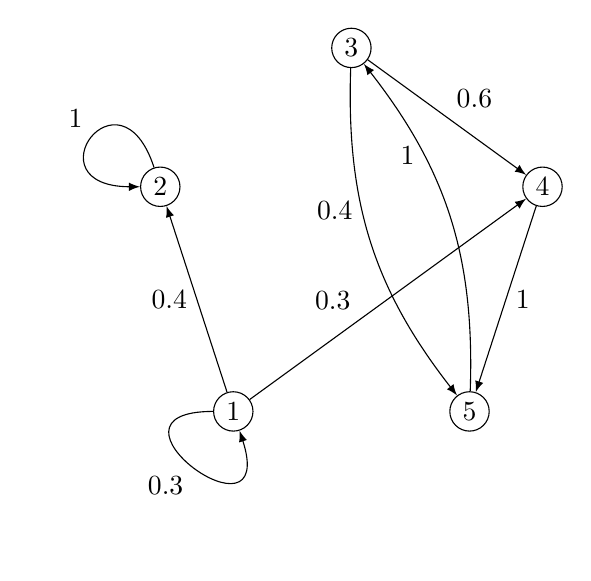
\begin{tikzpicture}[
    vertex/.style={circle, draw, minimum size=0.5cm, inner sep=0pt},
    baseline=(current bounding box.center),
  ]
    \def\radius{2.551952}
    \node[vertex] (1) at (234:\radius) {$1$};
    \node[vertex] (2) at (162:\radius) {$2$};
    \node[vertex] (3) at (90:\radius) {$3$};
    \node[vertex] (4) at (18:\radius) {$4$};
    \node[vertex] (5) at (306:\radius) {$5$};

    \draw[-latex] (1) to[out=180, in=288, looseness=10]
    node[below left] {$0.3$} (1);
    \draw[-latex] (1) to node[left] {$0.4$} (2);
    \draw[-latex] (1) to node[pos=0.4, above left] {$0.3$} (4);
    \draw[-latex] (2) to[out=108, in=180, looseness=12]
    node[above left] {$1$} (2);
    \draw[-latex] (3) to node[above right] {$0.6$} (4);
    \draw[-latex] (3) to[bend right=20] node[pos=0.4, left] {$0.4$} (5);
    \draw[-latex] (4) to node[right] {$1$} (5);
    \draw[-latex] (5) to[bend right=20] node[pos=0.7, left] {$1$} (3);
  \end{tikzpicture}
\end{minipage}%
\begin{minipage}[c]{0.45\textwidth}
  \begin{equation}
    \mathcal{P} =
    \begin{pmatrix}
      0.3 & 0.4 &  0  &  0  & 0.3 \\
      0  &  1  &  0  &  0  &  0  \\
      0  &  0  &  0  & 0.6 & 0.4 \\
      0  &  0  &  0  &  0  &  1  \\
      0  &  0  &  1  &  0  &  0
    \end{pmatrix}
  \end{equation}
\end{minipage}

\section{Proving the irreducibility of a chain}

Let’s consider the Markov chain defined by the matrix
\begin{equation}
  \mathcal{P}_{1} =
  \begin{pmatrix}
    1/2 & 1/2 \\
    1  &  0
  \end{pmatrix}.
\end{equation}
Is it irreducible? For every pair of states but one, $(2, 2)$, the corresponding
entry in $\mathcal{P}_1$ is different from zero. So, we can directly reach $1$
from $1$ and $2$, and $2$ from $1$. We have to find a path of any length $n$
that starts from $2$ and comes back to $2$, i.e. a $n$ such that $p^{n}_{ij} >
0$. Let’s see:
\begin{equation}
  \mathcal{P}_{1}^{2} =
  \begin{pmatrix}
    3/4 & 1/2 \\
    1/2 & 1/2
  \end{pmatrix}.
\end{equation}
So, there is a path of length $2$ that starts from $2$ and ends back there –
indeed, we can go from $2$ to $1$ with probability $1$ and then from $1$ to $2$
with probability $1/2$. Therefore, the Markov chain described by $\mathcal{P}_1$
is irreducible.

To find $\mathcal{P}_1^{n}$, it is best to diagonalize the matrix first:
\begin{equation}
  \mathcal{P}_{1}^{n} = T \mathcal{D}^{n} T^{-1}.
\end{equation}
The transformation matrix is given by
\begin{equation}
  T =
  \begin{pmatrix}
    1 & 1 \\
    1 & -2
  \end{pmatrix},
\end{equation}
while the diagonal matrix to the $n$-th power is
\begin{equation}
  \mathcal{D}^{n} =
  \begin{pmatrix}
    1 & 0 \\
    0 & -1/2
  \end{pmatrix}^n
  =
  \begin{pmatrix}
    1 & 0 \\
    0 & (-2)^{-n}
  \end{pmatrix}.
\end{equation}
Putting all together we obtain
\begin{equation}
  \mathcal{P}_{1}^{n} =
  \begin{pmatrix}
    1 & 1 \\
    1 & -2
  \end{pmatrix}
  \begin{pmatrix}
    1 & 0 \\
    0 & 2^{-n}
  \end{pmatrix}
  \begin{pmatrix}
    2/3 & 1/3 \\
    1/3 & -1/3
  \end{pmatrix}
  =\frac{1}{3}
  \begin{pmatrix}
    2 + (-1)^{n} 2^{-n} & 1 - (-1)^{n} 2^{-n} \\
    2 - (-1)^{n} 2^{1-n} & 1 + (-1)^{n} 2^{1-n}
  \end{pmatrix}.
\end{equation}
In the limit $n\to \infty$ this becomes
\begin{equation}
  \lim_{n \to \infty} \mathcal{P}_{1}^{n} =
  \begin{pmatrix}
    2/3 & 1/3 \\
    2/3 & 1/3
  \end{pmatrix}.
\end{equation}

Now, for the second matrix:
\begin{equation}
  \mathcal{P}_{2} =
  \begin{pmatrix}
    0  &  0  &  1  \\
    0  &  1  &  0  \\
    1/4 &  0  & 3/4
  \end{pmatrix},
\end{equation}
let’s find directly $\mathcal{P}_2^{n}$. The transformation matrix is
\begin{equation}
  T =
  \begin{pmatrix}
    -4 & 1 & 0 \\
    0 & 0 & 1 \\
    1 & 1 & 0
  \end{pmatrix},
\end{equation}
while the diagonalized one to the $n$-th power is
\begin{equation}
  \mathcal{D}^{n} =
  \begin{pmatrix}
    -1/4 & 0 & 0 \\
    0 & 1 & 0 \\
    0 & 0 & 1
  \end{pmatrix}^n
  =
  \begin{pmatrix}
    (-1)^{n} 4^{-n} & 0 & 0 \\
    0 & 1 & 0 \\
    0 & 0 & 1
  \end{pmatrix}.
\end{equation}
Putting everything together,
\begin{equation}
  \begin{split}
    \mathcal{P}_2^{n} &=
    \begin{pmatrix}
      -4 & 1 & 0 \\
      0 & 0 & 1 \\
      1 & 1 & 0
    \end{pmatrix}\,
    \begin{pmatrix}
      (-1)^{n} 4^{-n} & 0 & 0 \\
      0 & 1 & 0 \\
      0 & 0 & 1
    \end{pmatrix}\,
    \begin{pmatrix}
      -1/5 & 0 & 1/5 \\
      1/5 & 0 & 4/5 \\
      0 & 1 & 0
    \end{pmatrix} \\[1ex]
                      &= \frac{1}{5}
                      \begin{pmatrix}
                        1 + (-1)^{n} 4^{1-n} & 0 & 4 - (-1)^{n} 4^{1-n} \\
                        0 & 5 & 0 \\
                        1 - (-1)^{n} 4^{-n} & 0 & 4 + (-1)^{n} 4^{-n}
                      \end{pmatrix}.
  \end{split}
\end{equation}
Therefore, since $\mathcal{P}_{2}^{n}$ has entries which are zero, the
corresponding chain is \emph{not} irreducible. The limit $n \to \infty$ is
\begin{equation}
  \lim_{n \to \infty} \mathcal{P}_{2}^{n} =
  \begin{pmatrix}
    1/5 & 0 & 4/5 \\
    0 & 1 & 0 \\
    1/5 & 0 & 4/5
  \end{pmatrix}.
\end{equation}

\section{Proving the regularity of a chain}
The goal here is to prove whether the Markov chain defined by a given matrix is
regular. To do it, it suffices to find a $n$ such that every entry of
$\mathcal{P}^{n}$ is positive. This implies that every entry of
$\mathcal{P}^{m}$ is positive whenever $m \geq n$. In the first case it is
simple, $n = 2$ suffices to end the proof:
\begin{equation}
  \begin{pmatrix}
    1/2 & 1/4 & 1/4 \\
    1/2 &  0  & 1/2 \\
    1/4 & 1/4 & 1/2
  \end{pmatrix}^2
  = \frac{1}{16}
  \begin{pmatrix}
    7 & 3 & 6 \\
    6 & 4 & 6 \\
    6 & 3 & 7
  \end{pmatrix}.
\end{equation}

The second matrix instead is problematic:
\begin{equation}
  \begin{pmatrix}
    1 & 0 \\
    1/2 & 1/2
  \end{pmatrix}.
\end{equation}
If we look at it, we can realize that we cannot reach state $2$ from state $1$
in any way. So, the associated chain is reducible and irregular.

\section{Proving the stationarity of a chain}
In this exercise, the first stochastic matrix is
\begin{equation}
  \mathcal{P} =
  \begin{pmatrix}
    p  & 1-p &  0  &  0  \\
    0  &  0  &  p  & 1-p \\
    p  & 1-p &  0  &  0  \\
    0  &  0  &  p  & 1-p
  \end{pmatrix}.
\end{equation}
Let’s try to skip the calculations this time. If we consider state $1$, from the
first row we see that we can reach $2$ directly; from $2$ we can then reach $3$
and $4$. From $2$ we can reach $3$ and $4$; to reach $1$ we can pass through
$3$, since $p_{31} \neq 0$. $3$ and $4$ present the same situation as $1$ and
$2$ respectively. We can thus conclude that the associated Markov chain is
recurrent irreducible.

As for periodicity, if we square the matrix we get
\begin{equation}
  \mathcal{P}^{2} =
  \begin{pmatrix}
    p^{2} & p(1-p) & p(1-p) & (1-p)^{2} \\
    p^{2} & p(1-p) & p(1-p) & (1-p)^{2} \\
    p^{2} & p(1-p) & p(1-p) & (1-p)^{2} \\
    p^{2} & p(1-p) & p(1-p) & (1-p)^{2}
  \end{pmatrix},
\end{equation}
and this stays the same for all subsequent powers:
\begin{equation}
  \mathcal{P}^{3} =
  \begin{pmatrix}
    p^{2} & p(1-p) & p(1-p) & (1-p)^{2} \\
    p^{2} & p(1-p) & p(1-p) & (1-p)^{2} \\
    p^{2} & p(1-p) & p(1-p) & (1-p)^{2} \\
    p^{2} & p(1-p) & p(1-p) & (1-p)^{2}
  \end{pmatrix},
\end{equation}
and so on. So, the chain is definitely aperiodic, since all the entries of
$\mathcal{P}^{n}$ for $n > 1$ are positive.

To find the fixed point, we have to solve for $\pi$ the equation
\begin{equation}
  \pi \mathcal{P} = \pi \iff \mathcal{P}\tran \pi\tran = \pi\tran
  \iff (\mathcal{P}\tran - \I) \pi\tran = 0.
\end{equation}
This leads to the system of equations
\begin{equation}
  \begin{cases}
    (p-1)\pi_1 + \pi_3 = 0, \\
    (1-p)\pi_1 - \pi_2 +(1-p)\pi_3 = 0, \\
    p\pi_2 - \pi_3 + \pi_4 = 0, \\
    (1-p)\pi_2 - p\pi_4 = 0.
  \end{cases}
  \implies \dots \implies
  \begin{dcases}
    \pi_1 = \frac{p^{2}}{(1-p)^{2}}\pi_4, \\
    \pi_2 = \frac{p}{1-p}\pi_4, \\
    \pi_3 = \frac{p}{1-p}\pi_4.
  \end{dcases}
\end{equation}
Therefore, given a $q \in [0,1]$, the corresponding stationary $\pi$ is
\begin{equation}
  \pi_{q} = \left(\frac{p^{2}q}{(1-p)^{2}}, \frac{pq}{1-p}, \frac{pq}{1-p},
  q\right)
\end{equation}

The second part of the exercise asked to find another stationary distribution.
The matrix is
\begin{equation}
    \mathcal{P} =
    \begin{pmatrix}
        1/2 & 1/2 &  0  \\
        1/4 & 1/2 & 1/4 \\
         0  & 1/2 & 1/2
    \end{pmatrix}.
\end{equation}
The system corresponding to the equation $(\mathcal{P}\tran - \I) \pi\tran = 0$
is then
\begin{equation}
  \begin{pmatrix}
    -1/2 & 1/4 & 0 \\
    1/2 & -1/2 & 1/2 \\
    0 & 1/4 & -1/2
  \end{pmatrix}
  \begin{pmatrix}
    \pi_1 \\ \pi_2 \\ \pi_3 \\
  \end{pmatrix}
  =
  \begin{pmatrix}
    0 \\ 0 \\ 0
  \end{pmatrix}
  \implies
  \begin{cases}
    \pi_1 = \pi_3, \\
    \pi_2 = 2\pi_3.
  \end{cases}
\end{equation}
The stationary distribution is thus given by the state vectors
\begin{equation}
  \pi_q = (q, 2q, q) \quad\text{with } q \in [0, 1].
\end{equation}
